\documentclass[journal]{IEEEtran}
\usepackage[a5paper, margin=10mm]{geometry}
%\usepackage{lmodern} % Ensure lmodern is loaded for pdflatex
\usepackage{tfrupee} % Include tfrupee package


\setlength{\headheight}{1cm} % Set the height of the header box
\setlength{\headsep}{0mm}     % Set the distance between the header box and the top of the text


%\usepackage[a5paper, top=10mm, bottom=10mm, left=10mm, right=10mm]{geometry}

%
\setlength{\intextsep}{10pt} % Space between text and floats

\makeindex


\usepackage{cite}
\usepackage{amsmath,amssymb,amsfonts,amsthm}
\usepackage{algorithmic}
\usepackage{graphicx}
\usepackage{textcomp}
\usepackage{xcolor}
\usepackage{txfonts}
\usepackage{listings}
\usepackage{enumitem}
\usepackage{mathtools}
\usepackage{gensymb}
\usepackage{comment}
\usepackage[breaklinks=true]{hyperref}
\usepackage{tkz-euclide} 
\usepackage{listings}
\usepackage{multicol}
\usepackage{xparse}
\usepackage{gvv}
%\def\inputGnumericTable{}                                 
\usepackage[latin1]{inputenc}                  
\usepackage{color}                                            
\usepackage{array}                                          
\usepackage{longtable}                                       
\usepackage{calc}                                             
\usepackage{multirow}                                         
\usepackage{hhline}                                           
\usepackage{ifthen}                                     
\usepackage{lscape}
\usepackage{tabularx}
\usepackage{array}
\usepackage{float}
\usepackage{ar}
\usepackage[version=4]{mhchem}


\newtheorem{theorem}{Theorem}[section]
\newtheorem{problem}{Problem}
\newtheorem{proposition}{Proposition}[section]
\newtheorem{lemma}{Lemma}[section]
\newtheorem{corollary}[theorem]{Corollary}
\newtheorem{example}{Example}[section]
\newtheorem{definition}[problem]{Definition}
\newcommand{\BEQA}{\begin{eqnarray}}
\newcommand{\EEQA}{\end{endeqnarray}}

\theoremstyle{remark}


\begin{document}
\bibliographystyle{IEEEtran}
\onecolumn

\title{Graduate Aptitude Test in Engineering 2017 \\ Metallurgical Engineering}
\author{GATE 2017}
\maketitle


\renewcommand{\thefigure}{\theenumi}
\renewcommand{\thetable}{\theenumi}


\begin{enumerate}
\item For the matrix, 

\begin{align}
A= 
\myvec{1 & 1 & 2 \\ 2 & 1 & 1 \\1 & 1 & 2} , 
\end{align}
$AA^T $ is
\hfill{\brak{\text{GATE MT 2017}}}

\begin{multicols}{2}
\begin{enumerate}
    \item $\myvec{6 & 5 & 6 \\ 5 & 6 & 6 \\6 & 5 & 6}$
    \item $\myvec{6 & 5 & 6 \\ 5 & 6 & 6 \\5 & 5 & 6}$
    \item $\myvec{6 & 5 & 6 \\ 5 & 6 & 5 \\6 & 6 & 6}$
    \item $\myvec{6 & 5 & 6 \\ 5 & 6 & 5 \\6 & 5 & 6}$
\end{enumerate}
\end{multicols}

\item The mean of a numerical data-set is $\overline{X}$ and the standard deviation is S. If a number K is added to each term in the data-set then the mean and standard deviation become: \hfill{\brak{\text{GATE MT 2017}}}
\begin{multicols}{2}
\begin{enumerate}
    \item $\overline{X}$, S
    \item $\overline{X}+K$, S
    \item $\overline{X}$, $S+K$
    \item $\overline{X}+K$, $S+K$
\end{enumerate}
\end{multicols}

\item If $f(x)=e^{|x|}$ then at $x=0$, the function $f(x)$ is \hfill{\brak{\text{GATE MT 2017}}}
\begin{multicols}{2}
\begin{enumerate}
    \item continuous and differentiable.
    \item continuous but not differentiable.
    \item neither continuous nor differentiable.
    \item not continuous but differentiable.
\end{enumerate}
\end{multicols}

\item The pressure (P) versus volume (V) diagram given below represents reversible isothermal curves at temperatures, T1, T2 and T3.
\begin{figure}[H]
    \centering
    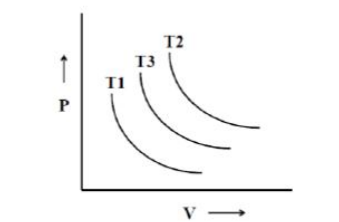
\includegraphics[width=0.4\columnwidth]{figs/Q.4.png}
    \caption\centering{REVERSIBLE ISOTHERMAL CURVES}
    \label{fig:placeholder}
\end{figure}
Considering one mole of ideal gas for all the three isothermal processes, which one of the following is TRUE? \hfill{\brak{\text{GATE MT 2017}}}
\begin{multicols}{2}
\begin{enumerate}
    \item $T1>T2>T3$
    \item $T2>T3>T1$
    \item $T3>T1>T2$
    \item $T2<T1<T3$
\end{enumerate}
\end{multicols}

\item For the electrochemical reaction, $Cu^{2+} + Zn = Zn^{2+} + Cu$, the standard cell potential at $25\degree\text{C}$ and 1 atm pressure is: (Given: $E\degree(\text{Cu}^{2+}/\text{Cu}) = 0.337 V$ and $E\degree(\text{Zn}^{2+}/\text{Zn}) = -0.763 V$) \hfill{\brak{\text{GATE MT 2017}}}
\begin{multicols}{4}
\begin{enumerate}
    \item $-0.426 V$
    \item $0.426 V$
    \item $0.55 V$
    \item $1.1 V$
\end{enumerate}
\end{multicols}

\item The rate of dissolution of Al particles in liquid steel is proportional to concentration difference $(\Delta C)$. $\Delta C$ is defined by:\\ (Given: (i) $C_b = $ bulk concentration of dissolved Al in liquid steel, (ii) $C^* = $ saturation concentration of Al in liquid steel at the given temperature, (iii) $C_m = $ Density of Al/Atomic weight of Al.) \hfill{\brak{\text{GATE MT 2017}}}
\begin{multicols}{4}
\begin{enumerate}
    \item $C^* - C_b$
    \item $C_b - C_m$
    \item $C^* - C_m$
    \item $\sqrt{C^*C_m} - C_b$
\end{enumerate}
\end{multicols}

\item Hydrogen dissolves in Pd by the reaction $H_2 = 2[H]$. At $300\degree\text{C}$ and $P_{H_2}=1$ atm, the solubility of hydrogen in Pd is $1.64 \times 10^4 \text{mm}^3$ (STP) per kg of Pd. At $300\degree\text{C}$ and $P_{H_2}=0.09$ atm, the solubility of hydrogen in Pd in $\text{mm}^3$ (STP) per kg of Pd is \underline {\hspace{2cm}} (answer up to one decimal place). \hfill{\brak{\text{GATE MT 2017}}}

\item The sieve analysis of ground quartz particles is given in the table below:
\begin{center}
\begin{tabular}{|c|c|}
\hline
\textbf{Sieve size (mm)} & \textbf{Mass fraction of ground product} \\
& \textbf{retained on each sieve} \\
\hline
4.76 & 0.0 \\
3.36 & 0.2 \\
2.38 & 0.4 \\
1.68 & 0.3 \\
1.19 & 0.08 \\
$<$1.19 & 0.02 \\
\hline
\end{tabular}
\end{center}
The cumulative mass fraction of particles of size less than 1.68 mm is \underline {\hspace{2cm}} (answer up to two decimal places). \hfill{\brak{\text{GATE MT 2017}}}

\item The sequence of precipitation to reach stable equilibrium during ageing of $Al-4.5 wt.\%$ Cu alloy is: \hfill{\brak{\text{GATE MT 2017}}}
\begin{multicols}{2}
\begin{enumerate}
    \item GP zone $\rightarrow \theta' \rightarrow \theta'' \rightarrow \theta$
    \item GP zone $\rightarrow \theta'' \rightarrow \theta' \rightarrow \theta$
    \item GP zone $\rightarrow \theta \rightarrow \theta'' \rightarrow \theta'$
    \item GP zone $\rightarrow \theta'' \rightarrow \theta \rightarrow \theta'$
\end{enumerate}
\end{multicols}

\item Tungsten powder is pressed at $150 MPa$ to a green density of $55\%$. After sintering, the compact attains $86.5\%$ of its theoretical density. Assuming uniform shrinkage, the linear shrinkage $(in \%)$ is \underline {\hspace{2cm}} (answer up to two decimal places). \hfill{\brak{\text{GATE MT 2017}}}

\item For a FCC metal, radius of the largest sphere that can fit in the tetrahedral void (in nm) is \underline {\hspace{2cm}} (answer up to three decimal places). (Given: lattice parameter = $0.401 nm$) \hfill{\brak{\text{GATE MT 2017}}}

\item In an iron-carbon alloy containing $0.35 wt.\% C$, the mass fraction of pearlite just below the eutectoid temperature is \underline {\hspace{2cm}} (answer up to two decimal places). (Given: eutectoid composition = $0.8 wt.\%$ carbon; and carbon content in ferrite is $0.025 wt.\%$) \hfill{\brak{\text{GATE MT 2017}}}

\item A cubic metal has a density of $19000 \text{ kg.m}^{-3}$, lattice parameter of $0.4 nm$ and atomic weight of 183. The effective number of atoms in an unit cell of this metal is \underline {\hspace{2cm}}. \hfill{\brak{\text{GATE MT 2017}}}

\item Primary mechanisms of accommodating plastic strain at low temperatures in crystalline metals are: \hfill{\brak{\text{GATE MT 2017}}}
\begin{multicols}{2}
\begin{enumerate}
    \item twinning and dislocation-slip
    \item dislocation-climb and dislocation-slip
    \item dislocation-slip and diffusion
    \item viscous-flow and dislocation-slip
\end{enumerate}
\end{multicols}

\item Spherical $\alpha$ phase particles are depicted in the hypothetical microstructure section shown below.
\begin{figure}[H]
    \centering
    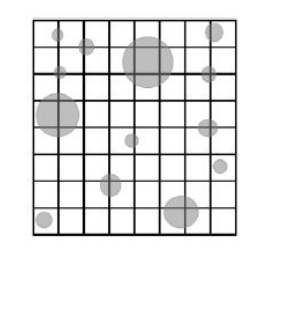
\includegraphics[width=0.3\columnwidth]{figs/Q.15.png}
    \caption\centering{MICROSTRUCTURE SECTION}
    \label{fig:placeholder}
\end{figure}
Using the superimposed grid on the microstructure, the estimated volume fraction of $\alpha$ phase is \underline {\hspace{2cm}} (answer up to three decimal places). \hfill{\brak{\text{GATE MT 2017}}}

\item A brittle material (Young's modulus = $60 GPa$ and surface energy = $0.5 \text{ J.m}^{-2}$) has a surface crack of length $2\micro m$. The fracture strength (in MPa) of this material is \underline {\hspace{2cm}} (answer up to two decimal places). \hfill{\brak{\text{GATE MT 2017}}}

\item Both creep resistance and tensile strength of a metal can be enhanced by \hfill{\brak{\text{GATE MT 2017}}}
\begin{multicols}{2}
\begin{enumerate}
    \item increase in the grain size
    \item decrease in the grain size
    \item addition of dispersoids
    \item annealing
\end{enumerate}
\end{multicols}

\item Stress required to operate a Frank-Read source of length L is approximately given by: \hfill{\brak{\text{GATE MT 2017}}}
\begin{multicols}{4}
\begin{enumerate}
    \item $\frac{Gb}{L}$
    \item $\frac{Gb^2}{L}$
    \item $\frac{Gb^2}{L^2}$
    \item $\frac{Gb^2}{2L^2}$
\end{enumerate}
\end{multicols}

\item The second peak in the powder X-ray diffraction pattern of a FCC metal occurs at a Bragg angle (in degrees) = \underline {\hspace{2cm}} (answer up to two decimal places). (Given: $\lambda_{CuK\alpha} = 0.154 nm$, lattice parameter of the metal = $0.36 nm$) \hfill{\brak{\text{GATE MT 2017}}}

\item A rod is elastically deformed by a uniaxial stress resulting in a strain of $0.02$. If the Poisson's ratio is $0.3$, the volumetric strain is \underline {\hspace{2cm}} (answer up to three decimal places). \hfill{\brak{\text{GATE MT 2017}}}

\item Four alloys, C1, C2, C3, C4, shown in the phase diagram are poured at temperature $T_1$ in a mold.
\begin{figure}[H]
    \centering
    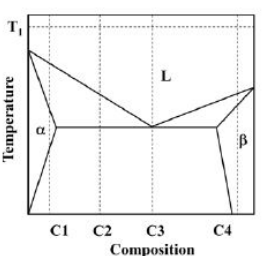
\includegraphics[width=0.3\columnwidth]{figs/Q.21.png}
    \caption\centering{PHASE DIAGRAM}
    \label{fig:placeholder}
\end{figure}
During solidification, which one of these alloys is expected to have the highest fluidity? \hfill{\brak{\text{GATE MT 2017}}}
\begin{multicols}{4}
\begin{enumerate}
    \item C1
    \item C2
    \item C3
    \item C4
\end{enumerate}
\end{multicols}

\item A material, which shows power law behavior, $\overline{\sigma}=50\overline{\epsilon}^{0.3}$, is being wire drawn. The maximum strain per pass in annealed condition (assume ideal work and efficiency $\eta=1$) is \underline {\hspace{2cm}} (answer up to two decimal places). \hfill{\brak{\text{GATE MT 2017}}}

\item Schematic diagram shows rolling of a slab. P and Q are points on the surface of the workpiece near entrance and exit, respectively.With reference to the work piece, which one of the following statements is TRUE?
\begin{figure}[H]
    \centering
    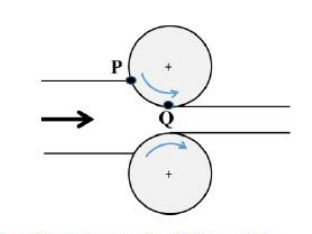
\includegraphics[width=0.4\columnwidth]{figs/Q.23.png}
    \caption\centering{ROLLING OF A SLAB}
    \label{fig:placeholder}
\end{figure}
 \hfill{\brak{\text{GATE MT 2017}}}
\begin{enumerate}
    \item Frictional force is along rolling direction at both P and Q.
    \item Frictional force is opposite to rolling direction at both P and Q.
    \item Frictional force is along rolling direction at P and opposite to rolling direction at Q.
    \item Frictional force is opposite to rolling direction at P and along rolling direction at Q.
\end{enumerate}

\item Which one of the following manufacturing techniques is used for making window glass? \hfill{\brak{\text{GATE MT 2017}}}
\begin{multicols}{2}
\begin{enumerate}
    \item Investment casting
    \item Patenting
    \item Spray forming
    \item Float-bath method
\end{enumerate}
\end{multicols}

\item Dye penetrant test is based on the principle of \hfill{\brak{\text{GATE MT 2017}}}
\begin{multicols}{2}
\begin{enumerate}
    \item polarized sound waves in liquid.
    \item magnetic domain.
    \item absorption of X-rays.
    \item capillary action.
\end{enumerate}
\end{multicols}



\item Assume that the probability of South Africa winning against India is $1/3$. If South Africa plays a 3 match cricket series against India, the probability that South Africa wins only one match is \underline {\hspace{2cm}} (assume that no matches are tied or abandoned) (answer up to three decimal places). \hfill{\brak{\text{GATE MT 2017}}}

\item The function $f(x)=x^3-3x$ has a minimum at $x=$ \underline {\hspace{2cm}}. \hfill{\brak{\text{GATE MT 2017}}}

\item The definite integral, $\int_{0}^{1}e^{-x^{2}}dx$ is to be evaluated numerically. Divide the integration interval into exactly 2 subintervals of equal length. Applying the trapezoidal rule, the approximate value of the integral is \underline {\hspace{2cm}} (answer up to two decimal places). \hfill{\brak{\text{GATE MT 2017}}}

\item For the second order linear ordinary differential equation,
\begin{align}
\frac{d^{2}y}{dx^{2}}+p\frac{dy}{dx}+qy=0,
\end{align}
the following function is a solution: $y=e^{\lambda x}$. Which one of the following statements is NOT TRUE? \hfill{\brak{\text{GATE MT 2017}}}

\begin{enumerate}
    \item $\lambda$ has two values: one complex and one real
    \item $\lambda^2 + p\lambda + q = 0$
    \item $\lambda$ has two real values
    \item $\lambda$ has two complex values
\end{enumerate}


\item Using the bisection method, the root of the equation $x^3+x-1=0$ after three iterations is \underline {\hspace{2cm}} (answer up to two decimal places). (Assume starting values of $x=-1$ and $+1$) \hfill{\brak{\text{GATE MT 2017}}}

\item $T_1$ and $T_2$ are the melting points of pure metal A and pure stoichiometric oxide $AO_2$, respectively, and $T_1 < T_2$. The stoichiometric metal oxidation reaction $A(s)+O_2(g)=AO_2(s)$ is in equilibrium at 1 atm pressure at temperature less than $T_1$. If the temperature increases, which schematic represents the correct standard free energy change versus temperature plot? \hfill{\brak{\text{GATE MT 2017}}}
\begin{figure}[H]
    \centering
    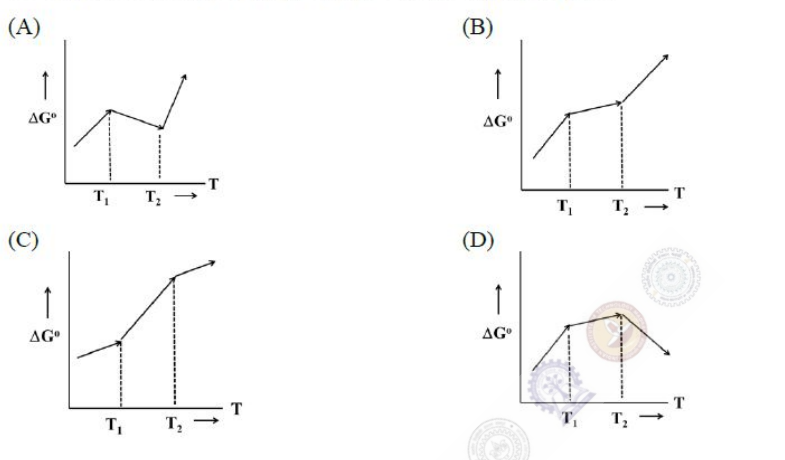
\includegraphics[width=0.8\columnwidth]{figs/Q.31.png}
    \caption\centering{SCHEMATIC DIAGRAM}
    \label{fig:placeholder}
\end{figure}
\item A continuous cast steel slab, $1m \times 1m \times 0.1m$, at 1298 K cools in air. The initial rate of heat loss (in kW) from the top surface of slab by radiation and convection is \underline {\hspace{2cm}} (answer up to two decimal places).\\
Given: (i) Ambient temperature = 298 K, (ii) emissivity of steel = 0.8, (iii) convective heat transfer coefficient = $4.6 \;\text{ W.m}^{-2}\text{.K}^{-1}$ (iv) Stefan-Boltzmann constant $(\sigma) = 5.7 \times 10^{-8} \text{W.m}^{-2}\text{.K}^{-4}$. \hfill{\brak{\text{GATE MT 2017}}}

\item The Pourbaix plot of the reaction $Al^{3+} + 2H2O = AlO2^{-} + 4H^{+}$ in potential (E) versus pH diagram is: \hfill{\brak{\text{GATE MT 2017}}}
\begin{figure}[H]
    \centering
    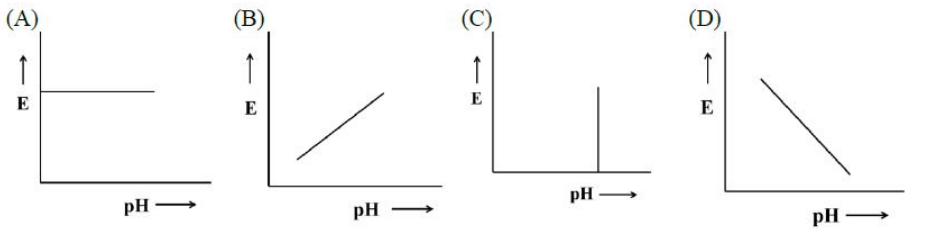
\includegraphics[width=0.9\columnwidth]{figs/Q.33.png}
    \caption\centering{POURBAIX PLOT}
    \label{fig:placeholder}
\end{figure}
\item During the end blow period in LD steelmaking, the de-carburization rate is expressed by the equation: $\frac{dc}{dt} = -(c-c^*)$. Here, $c$ and $c^*$ are the instantaneous and equilibrium concentration of carbon in steel respectively, in units of $wt.\%$. Given that $c^* = 0.04 wt.\%$ and $c(t=0 \text{ min}) = 0.4 wt.\%$, the concentration of carbon in steel $(in\;wt.\%)$ at t = 1 min is \underline {\hspace{2cm}} (answer up to three decimal places). \hfill{\brak{\text{GATE MT 2017}}}

\item $CaCO_3(s)$dissociates in a closed system according to the reaction
\begin{align}
CaCO_3(s) = CaO(s) + CO_2(g).
\end{align}
Assuming the reaction is in thermodynamic equilibrium, the degree(s) of freedom, F = \underline {\hspace{2cm}} \hfill{\brak{\text{GATE MT 2017}}}

\item A ladle containing molten steel is being discharged. The relevant forces are listed in Column I. Match them with their corresponding expressions in Column II. \hfill{\brak{\text{GATE MT 2017}}}
\begin{center}
\begin{tabular}{ll}
\textbf{Column I} & \textbf{Column II} \\
P.Pressure force & 1.$\mu UL$ \\
Q.Inertial force & 2.$\rho g L^3$ \\
R.Gravity force & 3.$\rho U^2 L^2$ \\
S. Viscous force & 4.$P L^2$ \\
\end{tabular}
\end{center}
$\mu=$ viscosity, $U=$ characteristic velocity, $L=$ characteristic length, $g=$ acceleration due to gravity, $P=$ pressure.
\begin{multicols}{2}
\begin{enumerate}
    \item $P-4, Q-3, R-2, S-1$
    \item $P-1, Q-3, R-2, S-4$
    \item $P-2, Q-3, R-4, S-1$
    \item $P-4, Q-3, R-1, S-2$
\end{enumerate}
\end{multicols}

\item In primary steelmaking, dissolved oxygen $(\underline{O})$ reacts with carbon $(\underline{C})$ to produce CO (g) at 1 atm pressure according to the reaction $\underline{C} + \underline{O} = CO(g)$. The equilibrium constant for this reaction is $\log K = \frac{1160}{T} + 2.003$, where T is in Kelvin. Assuming Henrian activity coefficient of both $\underline{O}$ and $\underline{C}$ to be unity, the dissolved oxygen content $(in\; wt.\%)$ of a plain carbon steel melt with $0.7\; wt.\% C$ at $1600\degree$C is \underline {\hspace{2cm}} (answer up to four decimal places). \hfill{\brak{\text{GATE MT 2017}}}

\item A stoichiometric mixture of CO and pure oxygen at 1 atm and $25\degree$C flows into a combustion reactor. The molar flow rate of CO entering the reactor is $1 kg-mol.h^{-1}$. The adiabatic flame temperature (in K) for the combustion of CO with stoichiometric oxygen is \underline {\hspace{2cm}} (answer up to two decimal places). Given: $\Delta H\degree_{298}(CO \rightarrow CO_2) = -282000 \text{ kJ.(kg-mol CO)}^{-1}$, $C_p(CO_2) = 44 \text{ kJ.(kg-mol.K)}^{-1}$. \hfill{\brak{\text{GATE MT 2017}}}

\item A solution contains $10^{-3}$ M of $Fe^{2+}$ at $25\degree$C. The solubility product of $Fe(OH)_3$ is $10^{-39}$. Assuming activity equals concentration, the minimum pH at which $Fe^{3+}$ will precipitate as $Fe(OH)_3$ is\underline {\hspace{2cm}} (answer up to two decimal places). \hfill{\brak{\text{GATE MT 2017}}}

\item A zinc electrowinning cell is being operated at a current of 400 A, voltage of 3.5 V, and a cathodic current efficiency of $90\%$. The specific energy consumption $(in \;MJ.kg^{-1}$ zinc) is \underline {\hspace{2cm}} (answer up to two decimal places). (Atomic weight of Zn=65) \hfill{\brak{\text{GATE MT 2017}}}

\item Pure metals A and B form two real binary solid solutions, $\alpha$ and $\beta$ at temperature T and pressure P. The free energy versus composition plots for both the solutions are shown below.
\begin{figure}[H]
    \centering
    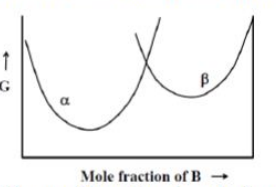
\includegraphics[width=0.4\columnwidth]{figs/Q.41.png}
    \caption\centering{FREE ENERGY VERSUS COMPOSITION PLOT}
    \label{fig:placeholder}
\end{figure}
The condition for chemical equilibrium is: \hfill{\brak{\text{GATE MT 2017}}}
\begin{enumerate}
    \item Mole fraction of A in $\alpha$ = mole fraction of A in $\beta$ and mole fraction of B in $\alpha$ = mole fraction of B in $\beta$
    \item Mole fraction of B in $\alpha$ = mole fraction of A in $\beta$ and mole fraction of A in $\alpha$ = mole fraction of B in $\beta$
    \item Activity of A in $\alpha$ = activity of A in $\beta$ and activity of B in $\alpha$ = activity of B in $\beta$
    \item Activity of A in $\alpha$ = activity of B in $\beta$ and activity of B in $\alpha$ = activity of A in $\beta$
\end{enumerate}

\item Pure orthorhombic sulfur transforms to stable monoclinic sulfur above 368.5 K. Applying Third law of thermodynamics, the value of entropy $(in\; J.K^{-1}$) of transformation at 368.5 K is \underline {\hspace{2cm}} (answer up to two decimal places). Given: (i) Entropy change associated with heating orthorhombic sulfur from 0 K to 368.5 K is 36.86 $J.K^{-1}$. (ii). Entropy change associated with cooling monoclinic sulfur from 368.5 K to 0 K is -37.8 $J.K^{-1}$. \hfill{\brak{\text{GATE MT 2017}}}

\item For homogeneous nucleation of solid in a liquid of a pure metal, the critical edge length (in nm) of a cube shaped nucleus is \underline {\hspace{2cm}} (answer up to two decimal places). (Given: surface energy $\gamma=0.177\text{ J.m}^{-2}$; change in volume free energy $\Delta G_V = -2.8 \times 10^8 \text{ J.m}^{-3}$) \hfill{\brak{\text{GATE MT 2017}}}

\item Assuming the solid phases to be pure, the slope of line BC in the predominance area diagram schematically shown below is \underline {\hspace{2cm}} (answer up to two decimal places).
\begin{figure}[H]
    \centering
    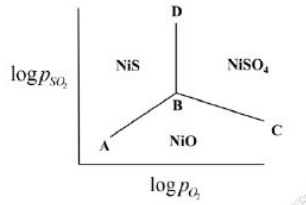
\includegraphics[width=0.4\columnwidth]{figs/Q.44.png}
    \caption\centering{SCHEMATIC DIAGRAM}
    \label{fig:placeholder}
\end{figure}
\hfill{\brak{\text{GATE MT 2017}}}

\item For each of the crystallographic system listed in Group-I, match the corresponding minimum symmetry in Group-II. \hfill{\brak{\text{GATE MT 2017}}}
\begin{center}
\begin{tabular}{ll}
\textbf{Group-I} & \textbf{Group-II} \\
P. Tetragonal & 1. 1 two-fold rotation \\
Q. Cubic & 2. 1 three-fold rotation \\
R. Monoclinic & 3. 4 three-fold rotation \\
S. Rhombohedral & 4. 1 four-fold rotation \\
\end{tabular}
\end{center}
\begin{multicols}{2}
\begin{enumerate}
    \item $P-3, Q-4, R-2, S-3$
    \item $P-4, Q-3, R-2, S-1$
    \item $P-1, Q-2, R-4, S-3$
    \item $P-4, Q-3, R-1, S-2$
\end{enumerate}
\end{multicols}

\item Arrange the magnetic moment of neighboring atoms in a one-dimensional lattice in Group-I to the corresponding magnetic material in Group-II. \hfill{\brak{\text{GATE MT 2017}}}
\begin{figure}[H]
    \centering
    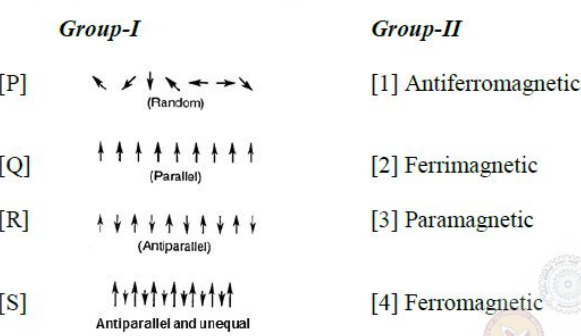
\includegraphics[width=0.7\columnwidth]{figs/Q.46.png}
    \caption\centering{ARRANGING MAGNETIC MOMENT}
    \label{fig:placeholder}
\end{figure}
\begin{multicols}{2}
\begin{enumerate}
    \item $P-4, Q-1, R-3, S-2$
    \item $P-3, Q-4, R-1, S-2$
    \item $P-2, Q-4, R-1, S-3$
    \item $P-1, Q-2, R-3, S-4$
\end{enumerate}
\end{multicols}

\item For an intrinsic semiconductor, the room temperature electrical conductivity is $10^{-6} \; \Omega^{-1}\text{.m}^{-1}$. If the electron and hole mobilities are 0.75 and $0.06 \text{ m}^2\text{.V}^{-1}\text{.s}^{-1}$ respectively, the intrinsic carrier concentration $(per\; m^3)$ at room temperature is \hfill{\brak{\text{GATE MT 2017}}}
\begin{multicols}{4}
\begin{enumerate}
    \item $5.1 \times 10^{12}$
    \item $7.7 \times 10^{12}$
    \item $8.3 \times 10^{12}$
    \item $1.1 \times 10^{14}$
\end{enumerate}
\end{multicols}

\item A steel component is subjected to fatigue loading, $\sigma(\text{maximum}) = 200$ MPa, $\sigma(\text{minimum}) = 0$. The component has an initial crack length of 1 mm. Propagation of crack is governed by 
\begin{align}
\frac{da}{dN}=10^{-12}(\Delta K)^3,
\end{align}
where the crack length $a$ is in meters, $N$ is the number of cycles and $\Delta K$ is in MPa.m$^{1/2}$. The length of the crack (in m) after one million cycles will be \underline {\hspace{2cm}}(answer up to three decimal places). \hfill{\brak{\text{GATE MT 2017}}}

\item During heat treatment of a cold worked metal , recrystallization is $20\%$ complete after 100s . The  transformation $(in\;\%)$ in 400s is \underline {\hspace{2cm}} (answer up to two decimal places)\\
(Assume Avrani exponent , n=2)
\hfill{\brak{\text{GATE MT 2017}}}


\item At low temperature, two parallel edge dislocations lying on parallel slip planes are shown in different configurations below.
\begin{figure}[H]
    \centering
    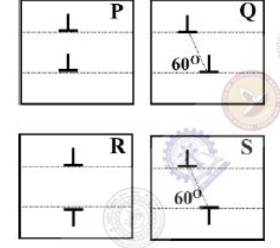
\includegraphics[width=0.5\columnwidth]{figs/Q.50.png}
    \caption\centering{DIFFERENT CONFIGURATIONS}
    \label{fig:placeholder}
\end{figure}
Match the following:
\begin{center}
\begin{tabular}{ll}
Configuration [P] & [1] Dislocations repel \\
Configuration [Q] & [2] Dislocations attract \\
Configuration [R] & [3] Dislocations are in stable equilibrium \\
Configuration [S] & [4] Dislocations are in unstable equilibrium \\
\end{tabular}
\end{center}
\begin{multicols}{2}
\begin{enumerate}
    \item P-3, Q-2, R-4, S-1
    \item P-4, Q-1, R-3, S-2
    \item P-1, Q-3, Q-2, R-4
    \item P-2, Q-4, R-1, S-3
\end{enumerate}
\end{multicols}

\item A single crystal of an FCC metal is subjected to a sufficiently large tensile stress along the $[110]$ direction to activate some of the slip systems . Which one of the following slip sysytems will be activated: \hfill{\brak{\text{GATE MT 2017}}}
\begin{multicols}{4}
\begin{enumerate}
    \item $\frac{a}{2}[\bar{1}10](111)$
    \item $\frac{a}{2}[01\bar{1}](1\bar{1}\bar{1})$
    \item $\frac{a}{2}[011](\bar{1}1\bar{1})$
    \item $\frac{a}{2}[1\bar{1}0](11\bar{1})$
\end{enumerate}
\end{multicols}

\item A perfectly elastic-plastic material has yield stress of 450 MPa  and fractures at a strain of 0.45 . The ratio of resilience to toughness of this material is \underline {\hspace{2cm}}(answer up to three decimal places )\\
(Given the Young's modulus E=4.5 GPa) \hfill{\brak{\text{GATE MT 2017}}}

\item Total time for solidification of a cubic casting of dimensions $5.0\text{ cm} \times 5.0\text{ cm} \times 5.0\text{ cm}$ is 1.6 min. A cylindrical riser with diameter to height ratio 0.5 is required so that the time for solidification of riser is 3.2 min. Applying Chvorinov's rule, the height of the riser (in cm) is\underline {\hspace{2cm}} (answer up to two decimal places). (Assume that exponent in Chvorinov's equation is 2) \hfill{\brak{\text{GATE MT 2017}}}

\item A 250 mm thick slab of a nickel alloy is subjected to cold rolling using a roll of diameter 450 mm. If the angle of bite during rolling is $10\degree$, the maximum possible reduction (in mm) during rolling is \underline {\hspace{2cm}} (answer up to two decimal places). \hfill{\brak{\text{GATE MT 2017}}}

\item W-Ni compact is prepared by liquid phase sintering at $1500\degree$C. If the size of tungsten grains is 40 \textmu m and the interfacial tungsten-tungsten and tungsten-nickel energies are 0.52 and $0.30 \text{ J.m}^{-2}$ respectively, the predicted average neck size (in \textmu m) of sintered tungsten grains is:\\ (Melting points of tungsten and nickel are $3410\degree$C and $1455\degree$C, respectively) \hfill{\brak{\text{GATE MT 2017}}}
\begin{multicols}{4}
\begin{enumerate}
    \item $10$
    \item $15$
    \item $20$
    \item $25$
\end{enumerate}
\end{multicols}



\item The ninth and the tenth of this month are Monday and Tuesday \underline {\hspace{2cm}}\hfill{\brak{\text{GATE MT 2017}}}
\begin{multicols}{4}
\begin{enumerate}
    \item figuratively
    \item retrospectively
    \item respectively
    \item rightfully
\end{enumerate}
\end{multicols}

\item It is \underline {\hspace{2cm}} to read this year's textbook \underline {\hspace{2cm}} the last year's. \hfill{\brak{\text{GATE MT 2017}}}
\begin{multicols}{4}
\begin{enumerate}
    \item easier, than
    \item most easy, than
    \item easier, from
    \item easiest, from
\end{enumerate}
\end{multicols}

\item A rule states that in order to drink beer, one must be over 18 years old. In a bar, there are 4 people. P is 16 years old, Q is 25 years old, R is drinking milkshake and S is drinking a beer. What must be checked to ensure that the rule is being followed? \hfill{\brak{\text{GATE MT 2017}}}
\begin{enumerate}
    \item Only P's drink
    \item Only P's drink and S's age
    \item Only S's age
    \item Only P's drink, Q's drink and S's age
\end{enumerate}

\item Fatima starts from point P, goes North for 3 km, and then East for 4 km to reach point Q. She then turns to face point P and goes 15 km in that direction. She then goes North for 6 km. How far is she from point P and in which direction should she go to reach point P? \hfill{\brak{\text{GATE MT 2017}}}
\begin{multicols}{4}
\begin{enumerate}
    \item 8 km, East
    \item 12 km, North
    \item 6 km, East
    \item 10 km, North
\end{enumerate}
\end{multicols}

\item 500 students are taking one or more courses out of Chemistry, Physics, and Mathematics. Registration records indicate course enrollment as follows: Chemistry (329), Physics (186), Mathematics (295), Chemistry and Physics (83), Chemistry and Mathematics (217), and Physics and Mathematics (63). How many students are taking all 3 subjects? \hfill{\brak{\text{GATE MT 2017}}}
\begin{multicols}{4}
\begin{enumerate}
    \item $37$
    \item $43$
    \item $47$
    \item $53$
\end{enumerate}
\end{multicols}

\item "If you are looking for a history of India, or for an account of the rise and fall of the British Raj, or for the reason of the cleaving of the subcontinent into two mutually antagonistic parts and the effects this mutilation will have in the respective sections, and ultimately on Asia, you will not find it in these pages; for though I have spent a lifetime in the country, I lived too near the seat of events, and was too intimately associated with the actors, to get the perspective needed for the impartial recording of these matters."\\ Which of the following statements best reflects the author's opinion? \hfill{\brak{\text{GATE MT 2017}}}
\begin{enumerate}
    \item An intimate association does not allow for the necessary perspective.
    \item Matters are recorded with an impartial perspective.
    \item An intimate association offers an impartial perspective.
    \item Actors are typically associated with the impartial recording of matters.
\end{enumerate}

\item Each of P, Q, R, S, W, X, Y and Z has been married at most once. X and Y are married and have two children P and Q. Z is the grandfather of the daughter S of P. Further, Z and W are married and are parents of R. Which one of the following must necessarily be FALSE? \hfill{\brak{\text{GATE MT 2017}}}
\begin{multicols}{2}
\begin{enumerate}
    \item X is the mother-in-law of R
    \item P and R are not married to each other
    \item P is a son of X and Y
    \item Q cannot be married to R
\end{enumerate}
\end{multicols}

\item 1200 men and 500 women can build a bridge in 2 weeks. 900 men and 250 women will take 3 weeks to build the same bridge. How many men will be needed to build the bridge in one week? \hfill{\brak{\text{GATE MT 2017}}}
\begin{multicols}{4}
\begin{enumerate}
    \item $3000$
    \item $3300$
    \item $3600$
    \item $3900$
\end{enumerate}
\end{multicols}

\item The number of 3-digit numbers such that the digit 1 is never to the immediate right of 2 is \hfill{\brak{\text{GATE MT 2017}}}
\begin{multicols}{4}
\begin{enumerate}
    \item $781$
    \item $791$
    \item $881$
    \item $891$
\end{enumerate}
\end{multicols}

\item A contour line joins locations having the same height above the mean sea level. The following is a contour plot of a geographical region. Contour lines are shown at 25 m intervals in this plot.
\begin{figure}[H]
    \centering
    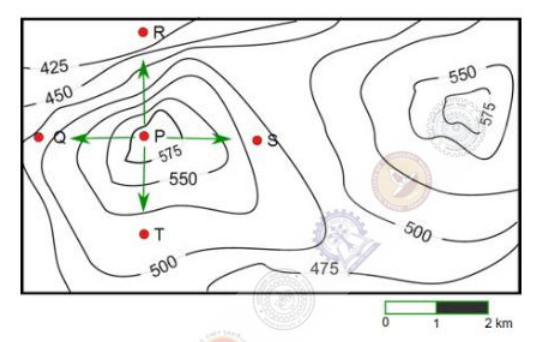
\includegraphics[width=0.6\columnwidth]{figs/Q.65.png}
    \caption\centering{CONTOUR PART OF A GEOGRAPHICAL REGION}
    \label{fig:placeholder}
\end{figure}
Which of the following is the steepest path leaving from P? \hfill{\brak{\text{GATE MT 2017}}}
\begin{multicols}{4}
\begin{enumerate}
    \item P to Q
    \item P to R
    \item P to S
    \item P to T
\end{enumerate}
\end{multicols}

\end{enumerate}
\section*{*END OF THE QUESTION PAPER*}
 
\end{document}